\chapter{Infrastructure}

The infrastructure of the hosted GitLab service in our OpenStack platform consists of:
\begin{itemize}
    \item n Runners (at the moment 1) in a separate 'gitlabrunners' network, which is not public accessible
    \item One public facing server which hosts GitLab itself in the 'provider' network,
          the Runners need to access this server via the 'gitlabrunners' network
\end{itemize}

\begin{figure}[H]
	\centering
	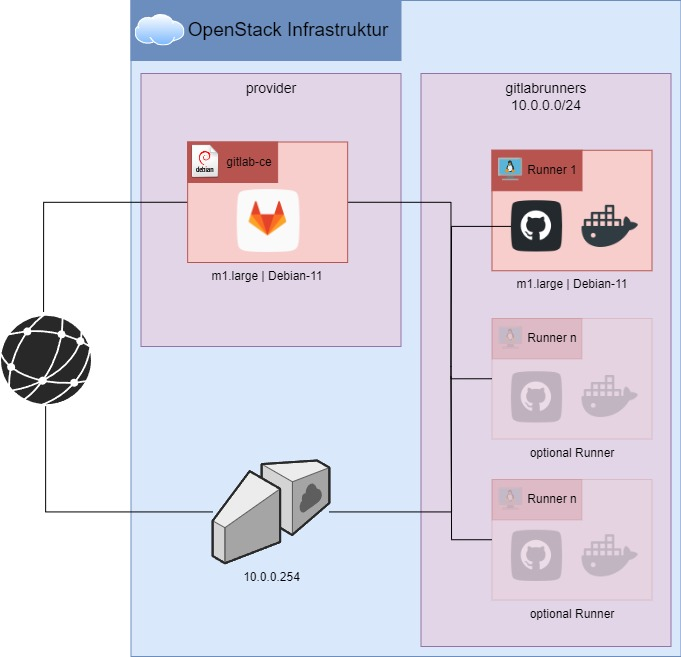
\includegraphics[width=12.5cm]{images/openstack_infrastructure.jpg}
	\caption{Infrastructure overview}
	\label{fig:openstack_infrastructure}
\end{figure}

\section{Networks}

The 'gitlabrunners' network has a network address of '10.0.0.0/24' and a gateway IP of '10.0.0.254'.
The DHCP range is defined as '10.0.0.100-10.0.0.200'.\\

The Runners need to access the internet, for installation of packages/updates, but also for getting data to be used in the CI process (e.g. getting Docker images). 
That is the reason why also a router is added for this network.

\subsection{Security Groups}

The following security groups are defined:
\begin{itemize}
    \item Default: do not open any inbound ports, allow outgoing traffic
    \item gitlab: Allow inbound traffic for HTTPS (tcp port 443) and GitLab Shell (tcp port 2224)
	\item SSH manage: Allow inbound traffic for SSH (tcp port 22)
\end{itemize}

\section{GitLab}

\subsection{Machine and network configuration} \label{gitlab_machine_network_configuration}

A machine named 'gitlab-ce' with flavor 'm1.large' and with 'Debian-11' as base image is used for the machine of the self-hosted GitLab instance.
This is due to CPU, memory and software requirements of GitLab and Docker.\\

A floating IP is leased and used for the 'provider' network.
Due to the availability of the domain 'gruber.info', an A-record for the \ac{fqdn} 'gitlabtest.gruber.info' is used (\ref{fig:a_record}) and an HTTPS certificate is generated for that \ac{fqdn} via Let´s encrypt (\ref{fig:lets_encrypt}) (\cite{refCloudflareCertbot}).
This certificate is used to prevent errors in the HTTPS communication.
\begin{figure}[H]
	\centering
	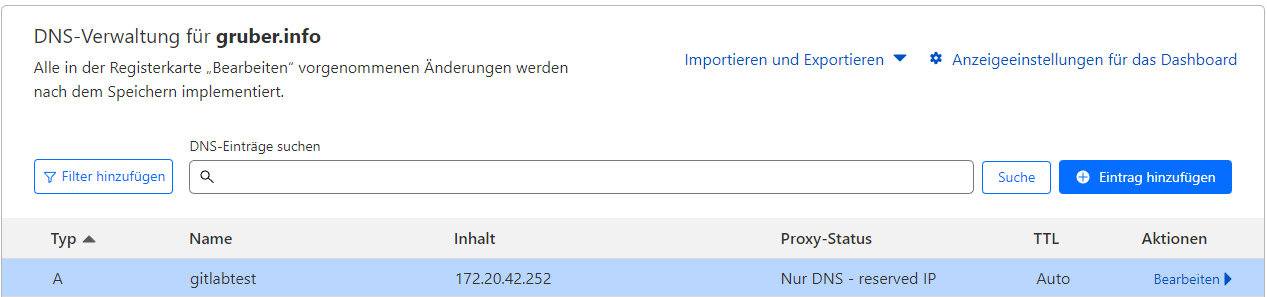
\includegraphics[width=14cm]{images/a-record.png}
	\caption{'gitlabtest.gruber.info' as A-record}
	\label{fig:a_record}
\end{figure}

\begin{figure}[H]
	\centering
	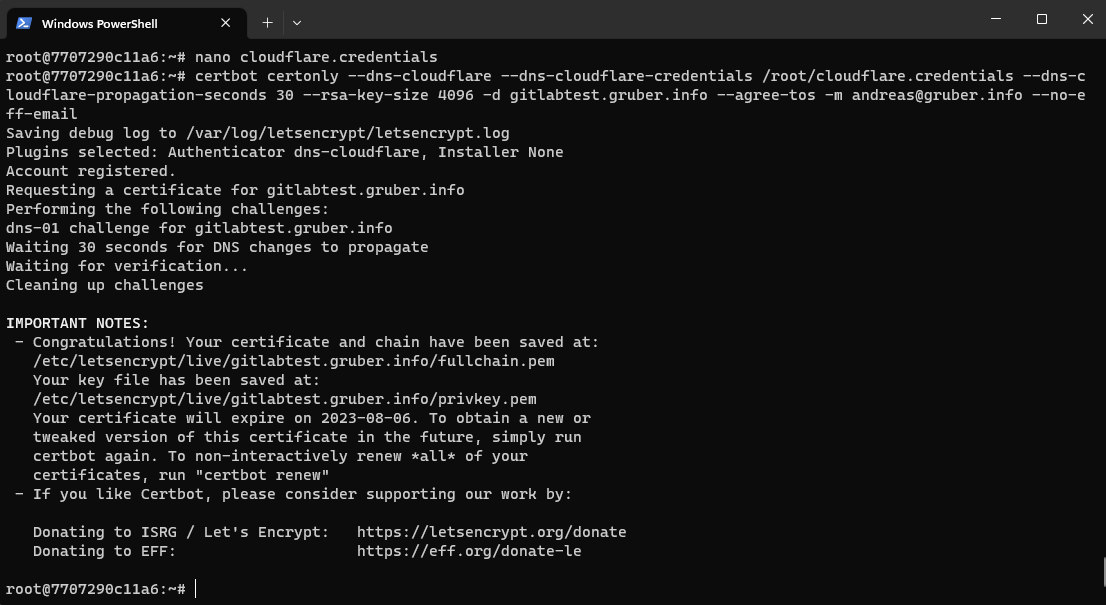
\includegraphics[width=14cm]{images/lets_encrypt.png}
	\caption{Let´s encrypt DNS-01 challenge}
	\label{fig:lets_encrypt}
\end{figure}

In the 'gitlabrunners' network a fixed IP of '10.0.0.99' is set for this machine, which can be used by the Runners to access GitLab.\\

The used security groups are 'Default' and 'gitlab'.\\

The 'SSH manage' security group is only enabled on demand when a login is required.

\subsection{OS configuration}

Login to the OS is only possible via SSH and SSH keys. Login with password is not possible.\\

As the 2GByte of memory is still not enough, a swap-file of 6GByte in size is added to the system (\ref{fig:swapfile}).
Without this, GitLab would not be able to start.

\begin{figure}[H]
	\centering
	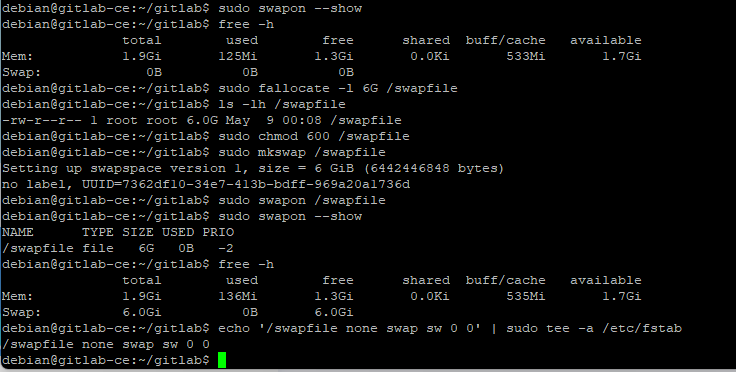
\includegraphics[width=14cm]{images/swapfile.png}
	\caption{Adding a swapfile}
	\label{fig:swapfile}
\end{figure}

Docker is installed according to the official Docker documentation (\cite{refDockerDebian}).

\section{GitLab Runners}

\subsection{Machine and network configuration}

A machine with flavor 'm1.large' with 'Debian-11' as base image is used for the machines of the self-hosted GitLab Runners.
At the time of the writing only 1 Runner is created and used.\\

The Runners get their IPs from the DHCP pool from the 'gitlabrunners' network.\\

The used security groups are 'Default' and 'SSH manage'.

\subsection{OS configuration}

Login to the OS is only possible via SSH and SSH keys. Login with password is not possible.\\

If access to the Internet fails, the reason might be that the nameservers are missing in the OS.
To solve such a problem an option is to add the following line to '/etc/resolv.conf':
\begin{lstlisting}
	nameserver 1.1.1.1
\end{lstlisting}
\  \\
Docker is installed according to the official Docker documentation (\cite{refDockerDebian}).\\

The Runners connect to the \ac{fqdn} of the GitLab host ('gitlabtest.gruber.info').
To make sure the Runners can access GitLab independent of the Internet, GitLab needs to be known to the Runners with its internal IP '10.0.0.99'.
This can be achieved for example by adding the following line to '/etc/hosts' on each Runner.
\begin{lstlisting}
10.0.0.99 gitlabtest.gruber.info
\end{lstlisting}
